\documentclass{beamer}
\usepackage{tikz}
\usetheme{Frankfurt}
\usecolortheme{seahorse}

\addtobeamertemplate{navigation symbols}{}{
    \usebeamerfont{footline}
    \usebeamercolor[fg]{footline}
    \hspace{1em}
    \raisebox{1.2pt}[0pt][0pt]{\insertframenumber/\inserttotalframenumber}
}

\setbeamertemplate{frametitle continuation}{%
    (\insertcontinuationcount)%
}

\title{DWA vs custom trajectory tracking controller}
\subtitle{A comparison in ROS}

\author[Chiari, Gargani, Salvi] {G. Chiari \and L. Gargani \and S. Salvi}
\institute {Politecnico di Milano}
\date {Academic Year 2022/2023}


\begin{document}

\begin{frame}
\titlepage
\end{frame}

\begin{frame}
\frametitle{Table of Contents}
\tableofcontents
\end{frame}

\AtBeginSection[]
{
  \begin{frame}
    \frametitle{Table of Contents}
    \tableofcontents[currentsection]
  \end{frame}
}



%-----------------------------------------------------------------------------
%                               INTRODUCTION
%-----------------------------------------------------------------------------

\section{Introduction}

% * * * * * * * * * * * * * * * * * * * * * * * * * * * * * * * * * * * * * * *

\begin{frame}
\frametitle{Frame title}

In this slide, some important text will be \alert{highlighted} because it's important.
Please, don't abuse it.

\begin{block}{Remark}
Sample text
\end{block}

\begin{alertblock}{Important theorem}
Sample text in red box
\end{alertblock}

\begin{examples}
Sample text in green box. The title of the block is ``Examples".
\end{examples}

\end{frame}

% * * * * * * * * * * * * * * * * * * * * * * * * * * * * * * * * * * * * * * *

\begin{frame}
\frametitle{Frame title}

\begin{columns}

\column{0.5\textwidth}
This is a text in first column.
$$E=mc^2$$
\begin{itemize}
	\item First item
	\item Second item
\end{itemize}

\column{0.5\textwidth}
This text will be in the second column and on a second thoughts, this is a nice looking layout in some cases.

\end{columns}

\end{frame}

% * * * * * * * * * * * * * * * * * * * * * * * * * * * * * * * * * * * * * * *

\begin{frame}
\frametitle{Project overview}

Test...

\end{frame}

% * * * * * * * * * * * * * * * * * * * * * * * * * * * * * * * * * * * * * * *

\begin{frame}
\frametitle{Differential drive}

Test...

\end{frame}


%-----------------------------------------------------------------------------
%                                   DWA
%-----------------------------------------------------------------------------

\section{DWA}

% * * * * * * * * * * * * * * * * * * * * * * * * * * * * * * * * * * * * * * *

\begin{frame}
\frametitle{Paper formulation}

Test...

\end{frame}

% * * * * * * * * * * * * * * * * * * * * * * * * * * * * * * * * * * * * * * *

\begin{frame}
\frametitle{ROS implementation}

Test...

\end{frame}



%-----------------------------------------------------------------------------
%                               CUSTOM CONTROLLER
%-----------------------------------------------------------------------------

\section{Custom controller}

% * * * * * * * * * * * * * * * * * * * * * * * * * * * * * * * * * * * * * * *

\begin{frame}
\frametitle{Unicycle model control}

Test...

\end{frame}

% * * * * * * * * * * * * * * * * * * * * * * * * * * * * * * * * * * * * * * *

\begin{frame}
\frametitle{Controller's architecture}

Test...

\end{frame}



%-----------------------------------------------------------------------------
%                                   THE EXPERIMENT
%-----------------------------------------------------------------------------

\section{The experiment}

% * * * * * * * * * * * * * * * * * * * * * * * * * * * * * * * * * * * * * * *

\begin{frame}
\frametitle{Experiment setup - the robot}

\begin{columns}

\column{0.5\textwidth}

The robot:
\begin{itemize}
  \item differential drive
  \item \texttt{d} = 15 cm (wheels distance)
  \item \texttt{r} = 3 cm (wheels radius)
  \item pentagonal footprint
\end{itemize}


\column{0.5\textwidth}

[IMAGE FROM RVIZ]

\end{columns}

\end{frame}

% * * * * * * * * * * * * * * * * * * * * * * * * * * * * * * * * * * * * * * *

\begin{frame}
\frametitle{Experiment setup - the map}

\begin{columns}

\column{0.6\textwidth}

The map:
\begin{itemize}
  \item empty, no obstacles around
  \item global, no need for a local one
\end{itemize}


\column{0.4\textwidth}

[IMAGE FROM RVIZ]

\end{columns}

\end{frame}

% * * * * * * * * * * * * * * * * * * * * * * * * * * * * * * * * * * * * * * *

\begin{frame}
\frametitle{Experiment setup - the trajectory}

\begin{columns}

\column{0.6\textwidth}

The trajectory:
\begin{itemize}
  \item eight-shaped
  \item 2 x 1 meters
  \item discretized into multiple goals
\end{itemize}


\column{0.4\textwidth}

[IMAGE FROM RVIZ]

\end{columns}

\end{frame}

% * * * * * * * * * * * * * * * * * * * * * * * * * * * * * * * * * * * * * * *

\begin{frame}[allowframebreaks]
\frametitle{ROS architecture - overview}

Three packages:
\begin{itemize}
  \item \texttt{diffdrive\_kin\_sim} $\rightarrow$ simulator
  \item \texttt{diffdrive\_kin\_ctrl} $\rightarrow$ custom controller
  \item \texttt{diffdrive\_dwa\_ctrl} $\rightarrow$ DWA controller
\end{itemize}

\vspace{2em}

The two controllers are interchangeable and are meant to always be used together
with the simulator, one at a time.

\framebreak

\begin{columns}

\column{0.5\textwidth}

\begin{figure}[H]
    \centering
    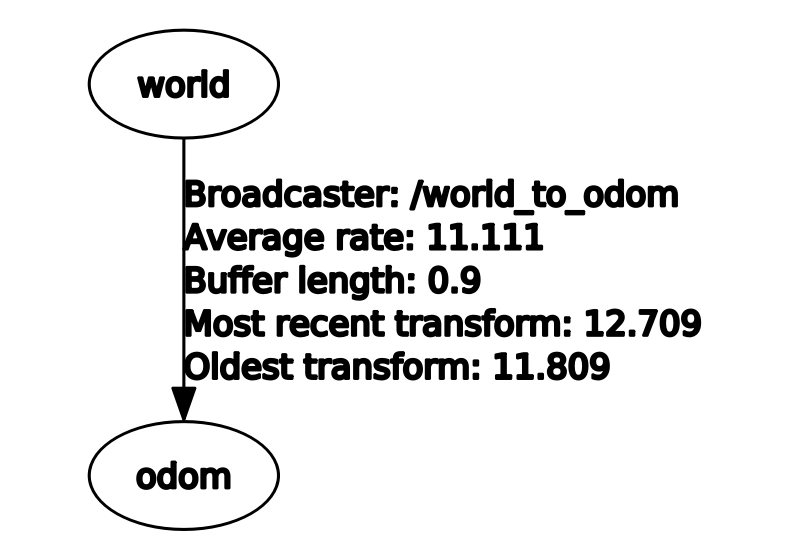
\includegraphics[scale=0.26]{img/ros_tools/rqttftree_custom.png}
\end{figure}

\column{0.5\textwidth}

\begin{figure}[H]
    \centering
    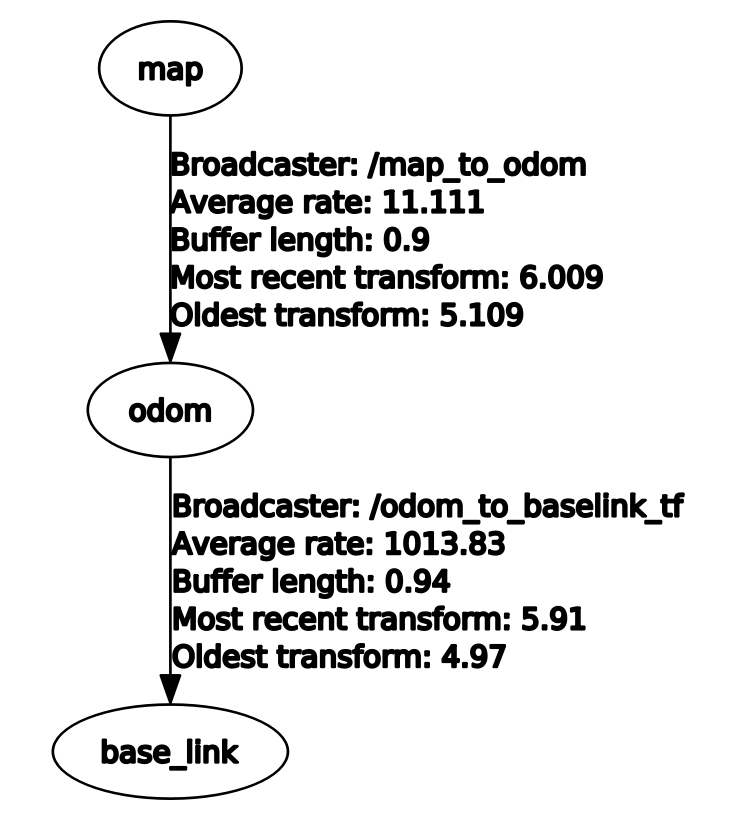
\includegraphics[scale=0.28]{img/ros_tools/rqttftree_dwa.png}
\end{figure}

\end{columns}

\end{frame}

% * * * * * * * * * * * * * * * * * * * * * * * * * * * * * * * * * * * * * * *

\begin{frame}[allowframebreaks]
\frametitle{ROS architecture - service \& frames}

One service:
\begin{itemize}
  \item \texttt{generate\_desired\_path\_service} $\rightarrow$ used to generate the eight-shaped trajectory as soon as it is invoked by one of the two controllers
\end{itemize}

\vspace{2em}

Three frames:
\begin{itemize}
  \item \texttt{map} $\rightarrow$ for the empty map provided by the map server
  \item \texttt{odom} $\rightarrow$ representing the global reference system
  \item \texttt{base\_link} $\rightarrow$ representing the moving reference system
\end{itemize}

\framebreak

\begin{figure}[H]
    \centering
    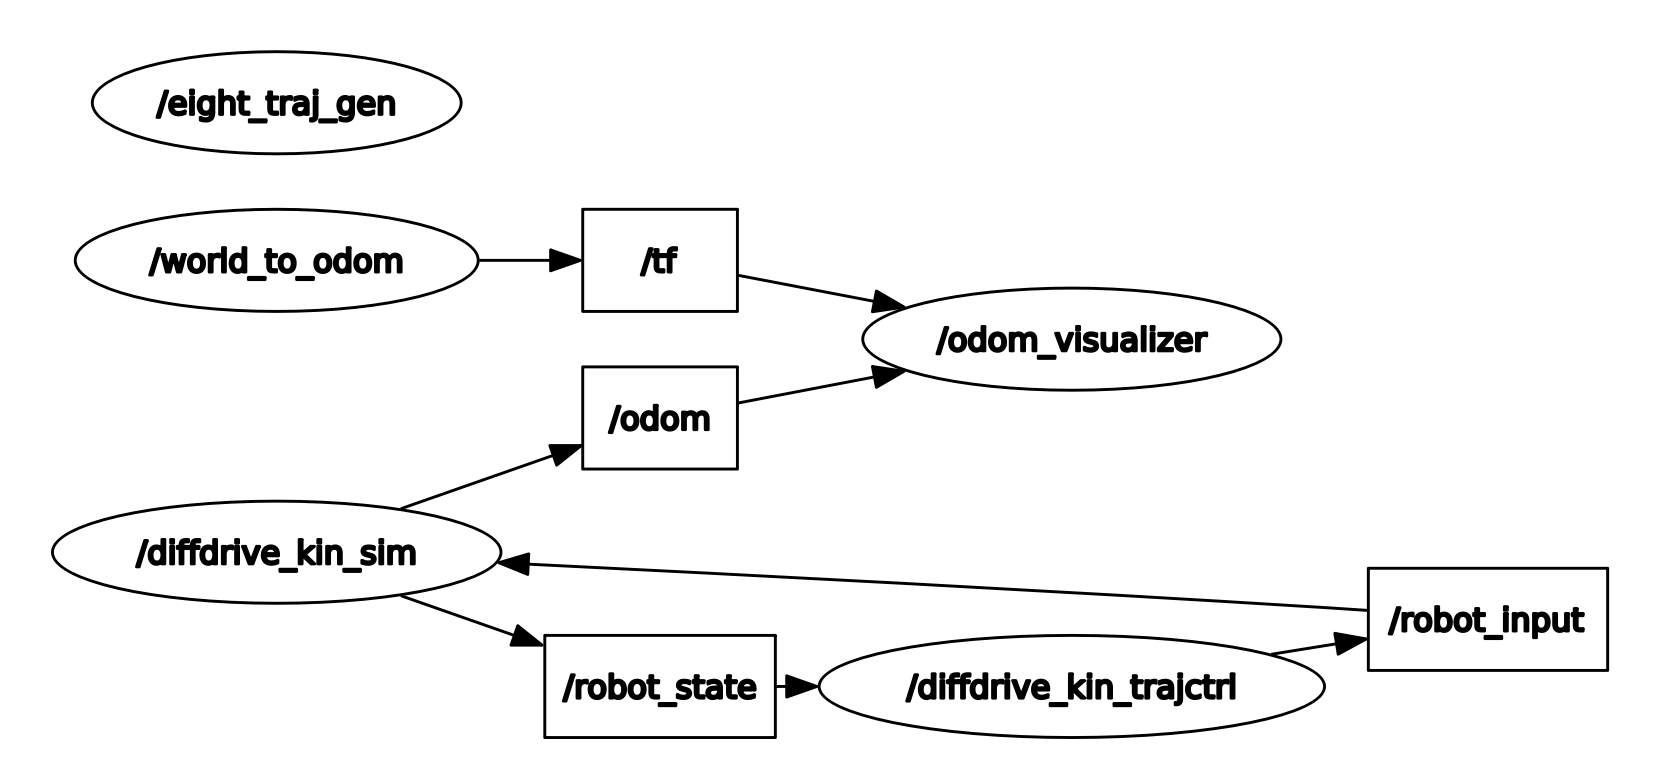
\includegraphics[scale=0.14]{img/ros_tools/rqtgraph_custom.png}
\end{figure}

\vspace{-2em}

\begin{figure}[H]
    \centering
    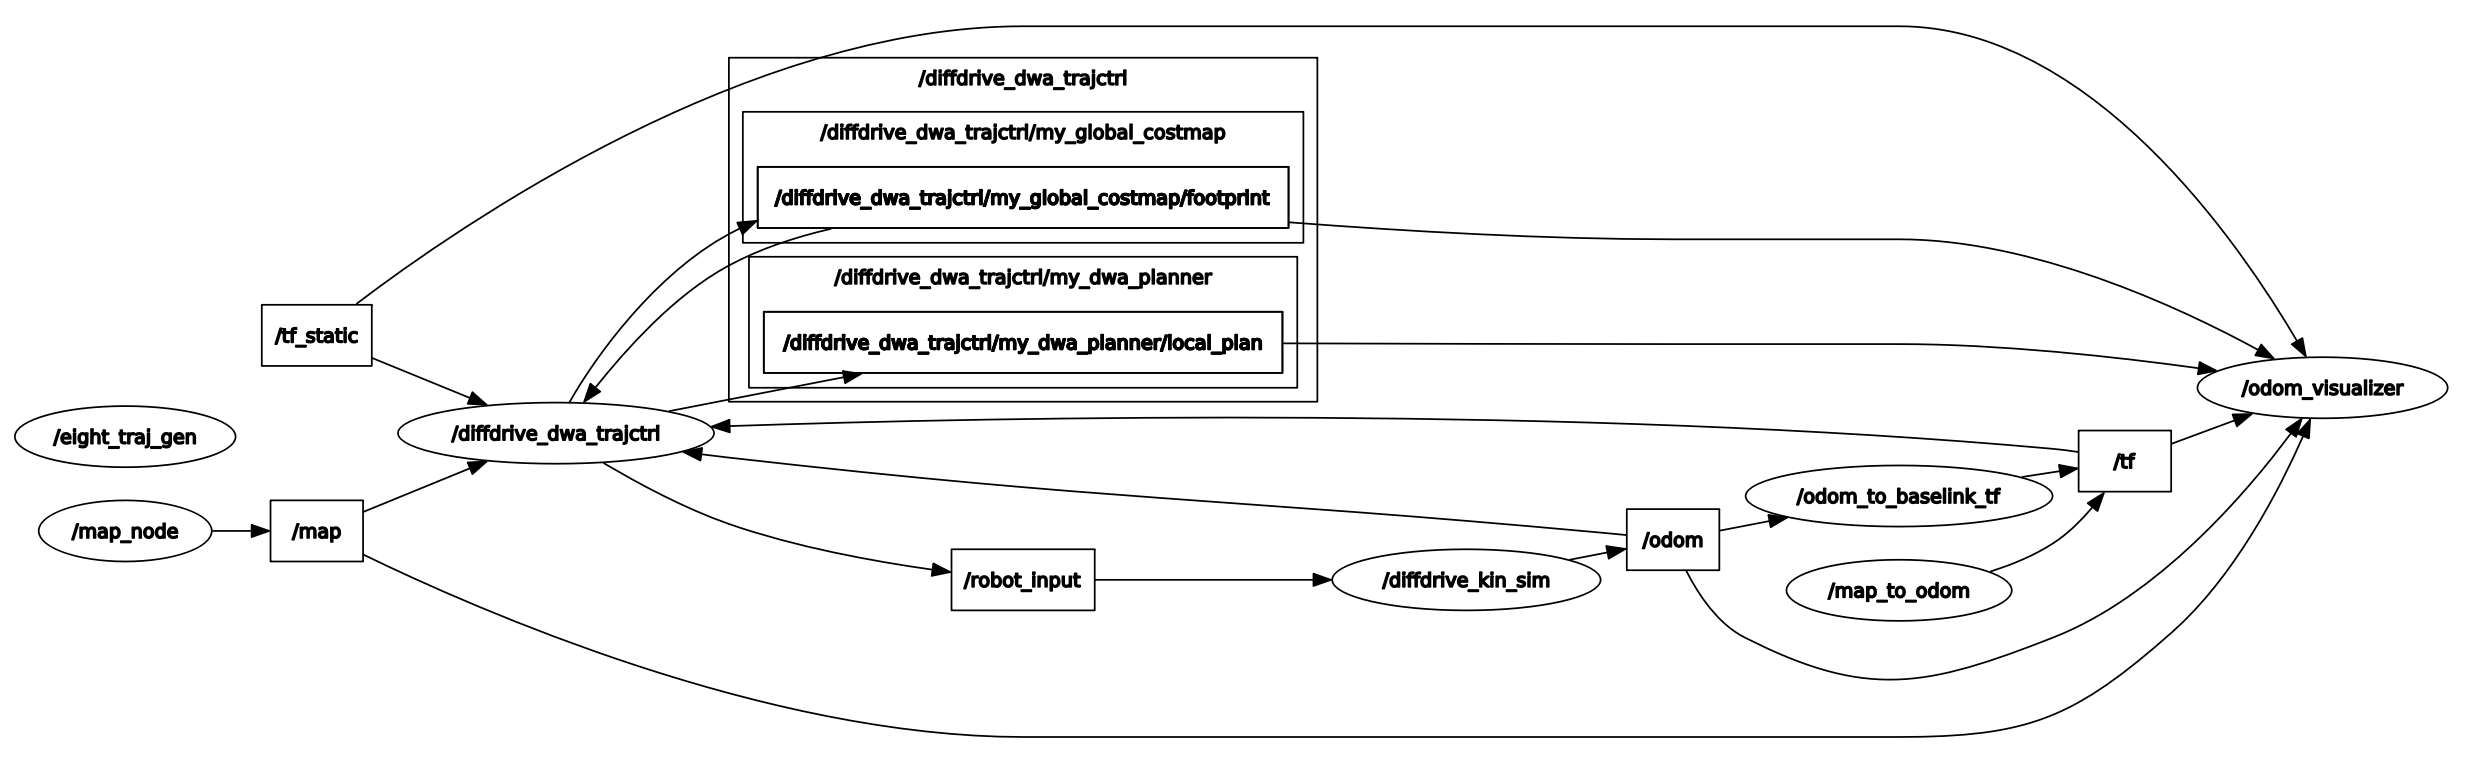
\includegraphics[scale=0.17]{img/ros_tools/rqtgraph_dwa.png}
\end{figure}

\end{frame}

% * * * * * * * * * * * * * * * * * * * * * * * * * * * * * * * * * * * * * * *

\begin{frame}
\frametitle{ROS architecture - nodes}

Four nodes:
\begin{itemize}
  \item \texttt{diffdrive\_kin\_sim\_node}, $\rightarrow$ integration logic to update the robot pose given ($\omega_r$,$\omega_l$)
  \item \texttt{diffdrive\_kin\_trajctrl\_node}, $\rightarrow$ computation of ($\omega_r$,$\omega_l$) to reach the next point in the trajectory, using the custom controller
  \item \texttt{diffdrive\_dwa\_trajctrl\_node}, $\rightarrow$ interface between DWA library and simulator to compute ($\omega_r$,$\omega_l$)
  \item \texttt{odom\_to\_baselink\_tf\_node}, link between the \texttt{odom} and the \texttt{base\_link} coordinate frames through a dynamic tf
\end{itemize}

\end{frame}

% * * * * * * * * * * * * * * * * * * * * * * * * * * * * * * * * * * * * * * *

\begin{frame}
\frametitle{ROS architecture - topics}

Four nodes:
\begin{itemize}
  \item \texttt{/clock}, $\rightarrow$ synchronization of all the nodes in the simulation
  \item \texttt{/odom}, $\rightarrow$ communication of the odometry information of the robot to DWA
  \item \texttt{/robot\_state}, $\rightarrow$ communication of the odometry information of the robot to the custom controller
  \item \texttt{/controller\_state}, $\rightarrow$ for visualization purposes
  \item \texttt{/robot\_input}, $\rightarrow$ communication of ($\omega_r$,$\omega_l$) computed by the controllers
\end{itemize}

\end{frame}

% * * * * * * * * * * * * * * * * * * * * * * * * * * * * * * * * * * * * * * *

\begin{frame}
\frametitle{ROS architecture - launch files}

Two launch files:
\begin{itemize}
  \item \texttt{diffdrive\_kin\_trajctrl.launch} $\rightarrow$ start the simulation of the robot's behavior with the custom controller
  \item \texttt{diffdrive\_dwa\_trajctrl.launch} $\rightarrow$ start the simulation of the robot's behavior with DWA
\end{itemize}


\end{frame}

% * * * * * * * * * * * * * * * * * * * * * * * * * * * * * * * * * * * * * * *

\begin{frame}
\frametitle{Parameters tuning - trajectory}

$$
\begin{cases}
    x = \texttt{a} \cdot \sin (\texttt{w} \cdot t)\\
    y = \texttt{a} \cdot \sin (\texttt{w} \cdot t)\cdot \cos (\texttt{w} \cdot t)\\
\end{cases}
$$

\vspace{2em}

Two main parameters:
\begin{itemize}
 \item \texttt{a} $\rightarrow$ amplitude of the eight-shaped trajectory
 \item \texttt{w} $\rightarrow$ ratio $\frac{2 \cdot \pi}{T}$ where T is the time duration of each lap
\end{itemize}

\vspace{2em}

\begin{block}{Assigned values}
\centering
\texttt{a} = 1
\hspace{3em}
\texttt{w} = 1
\end{block}

\end{frame}

% * * * * * * * * * * * * * * * * * * * * * * * * * * * * * * * * * * * * * * *

\begin{frame}
\frametitle{Parameters tuning - custom controller}

$$
u(t)=K_{\text{p}}e(t)+K_{\text{i}}\int _{0}^{t}e(\tau )\,\mathrm {d} \tau +K_{\text{d}}{\frac {\mathrm {d} e(t)}{\mathrm {d} t}}
$$

\vspace{2em}

Three main parameters:
\begin{itemize}
 \item $K_p$ $\rightarrow$ proportional gain of the PID controller
 \item $K_i$ $\rightarrow$ integral gain of the PID controller
 \item $K_d$ $\rightarrow$ derivative gain of the PID controller
\end{itemize}

\vspace{2em}

\begin{block}{Assigned values}
\centering
$K_p$ = 0.8
\hspace{3em}
$K_i$ = 0.8
\hspace{3em}
$K_d$ = 0.0
\end{block}

\end{frame}

% * * * * * * * * * * * * * * * * * * * * * * * * * * * * * * * * * * * * * * *

\begin{frame}
\frametitle{Parameters tuning - DWA}

One main parameter:
\begin{itemize}
  \item \texttt{skipped\_goals} $\rightarrow$ number of points to skip when feeding the trajectory to DWA
\end{itemize}

\vspace{2em}

\begin{block}{Assigned values}
\centering
\texttt{skipped\_goals} = 15
\end{block}

\end{frame}



%-----------------------------------------------------------------------------
%                             EXPERIMENTAL RESULTS
%-----------------------------------------------------------------------------

\section{Experimental results}


% * * * * * * * * * * * * * * * * * * * * * * * * * * * * * * * * * * * * * * *

\begin{frame}
\frametitle{Python scripts}

To visualize the experimental results of the experiment, two Python scripts can
be used to analyze the recorded \textit{bag} files:
\begin{itemize}
  \item \texttt{plot\_result.py} $\rightarrow$ plot the result of a single \textit{bag} file
  \item \texttt{plot\_comparison.py} $\rightarrow$ compare the results of two \textit{bag} files
\end{itemize}

\vspace{2em}

The following plots are obtained with an optimal parameters choice.

\end{frame}

% * * * * * * * * * * * * * * * * * * * * * * * * * * * * * * * * * * * * * * *

\begin{frame}[allowframebreaks]
\frametitle{Trajectory tracking controller}

\vspace{-2em}

\begin{figure}[H]
    \centering
    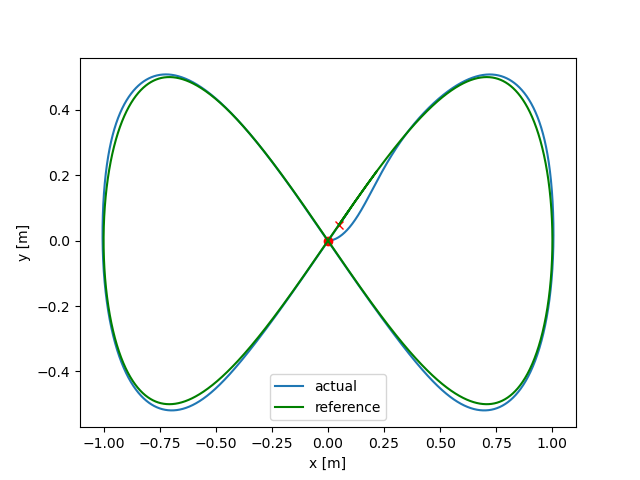
\includegraphics[scale=0.6]{img/kin_screenshots/Trajectory.png}
\end{figure}

\framebreak

\begin{columns}

\column{0.5\textwidth}

\vspace{-2em}

\begin{figure}[H]
    \centering
    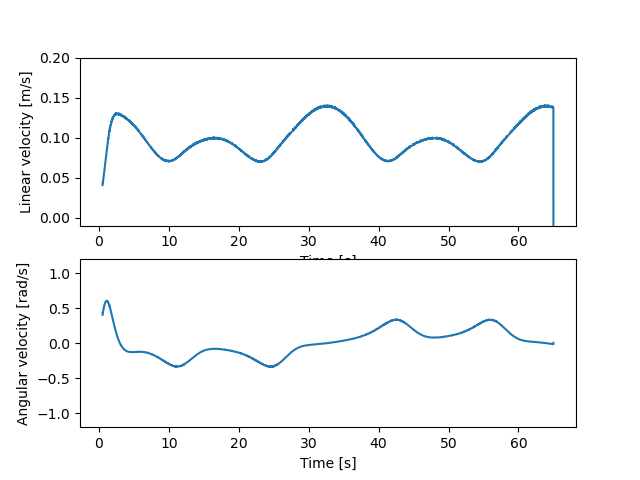
\includegraphics[scale=0.3]{img/kin_screenshots/Linear_and_Angular_Velocities.png}
\end{figure}

\vspace{-1em}

\begin{figure}[H]
    \centering
    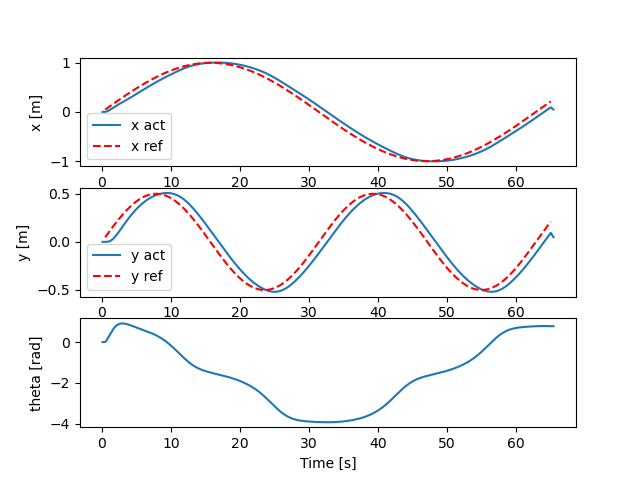
\includegraphics[scale=0.3]{img/kin_screenshots/Pose.png}
\end{figure}

\column{0.5\textwidth}

\vspace{-2em}

\begin{figure}[H]
    \centering
    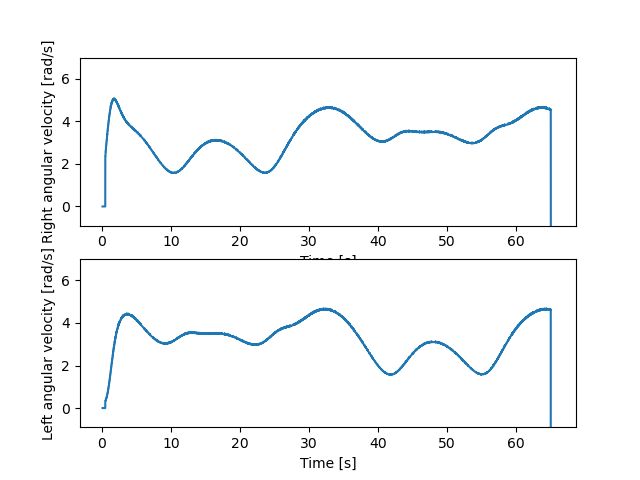
\includegraphics[scale=0.3]{img/kin_screenshots/Wheels_Velocities.png}
\end{figure}

\vspace{-1em}

\begin{figure}[H]
    \centering
    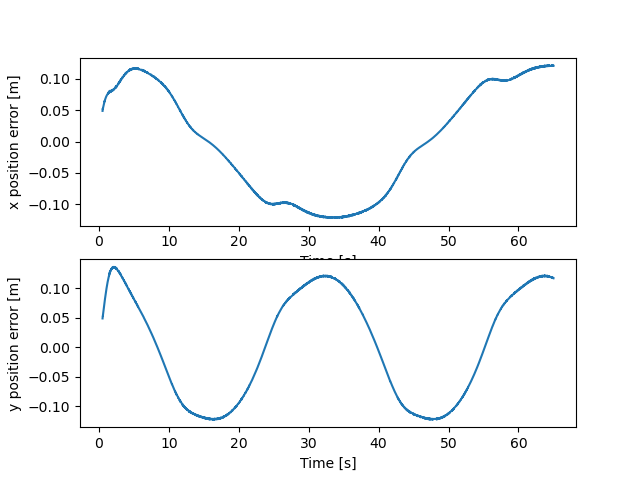
\includegraphics[scale=0.3]{img/kin_screenshots/Position_Error.png}
\end{figure}

\end{columns}

\end{frame}

% * * * * * * * * * * * * * * * * * * * * * * * * * * * * * * * * * * * * * * *

\begin{frame}[allowframebreaks]
\frametitle{DWA}

\vspace{-2em}

\begin{figure}[H]
    \centering
    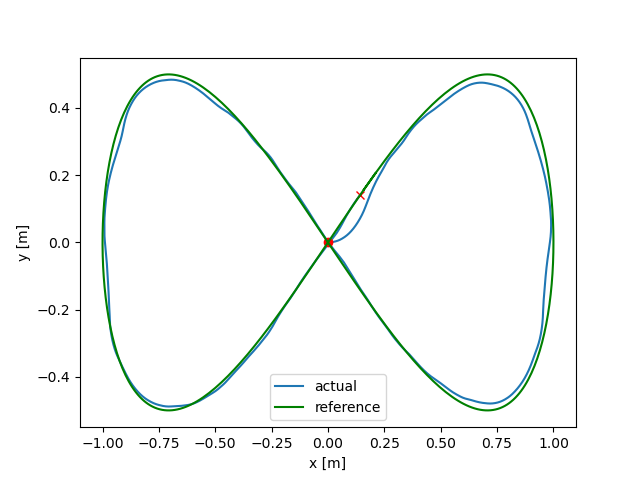
\includegraphics[scale=0.6]{img/dwa_screenshots/Trajectory.png}
\end{figure}

\framebreak

\begin{columns}

\column{0.5\textwidth}

\vspace{-2em}

\begin{figure}[H]
    \centering
    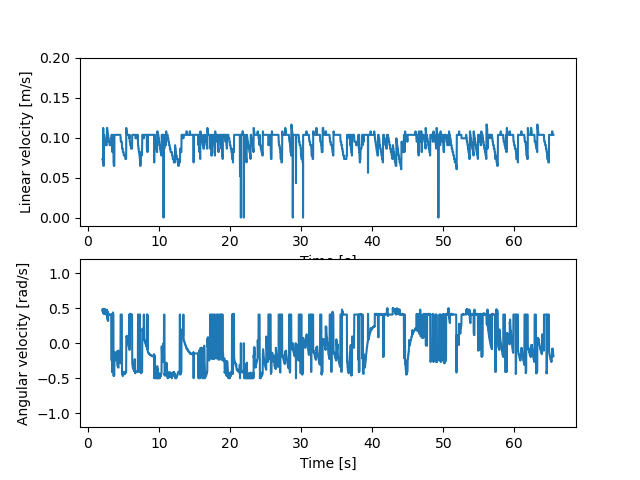
\includegraphics[scale=0.3]{img/dwa_screenshots/Linear_and_Angular_Velocities.png}
\end{figure}

\vspace{-1em}

\begin{figure}[H]
    \centering
    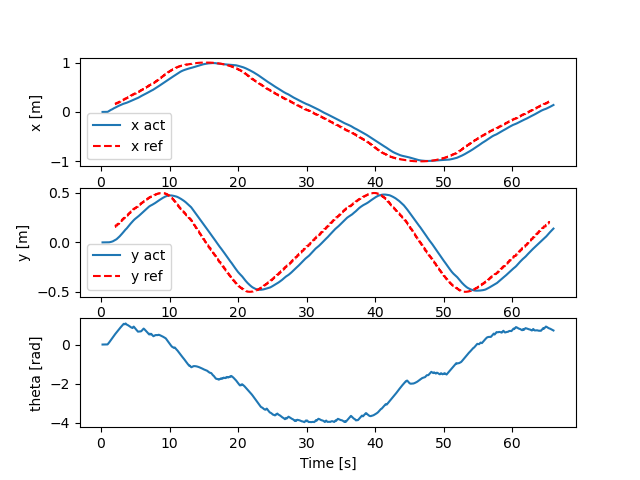
\includegraphics[scale=0.3]{img/dwa_screenshots/Pose.png}
\end{figure}

\column{0.5\textwidth}

\vspace{-2em}

\begin{figure}[H]
    \centering
    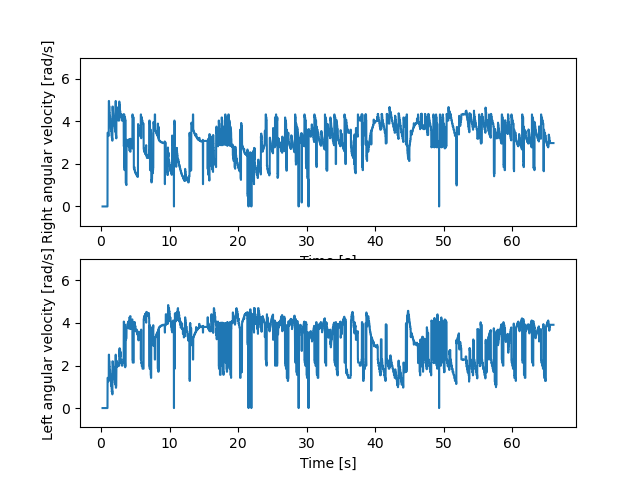
\includegraphics[scale=0.3]{img/dwa_screenshots/Wheels_Velocities.png}
\end{figure}

\vspace{-1em}

\begin{figure}[H]
    \centering
    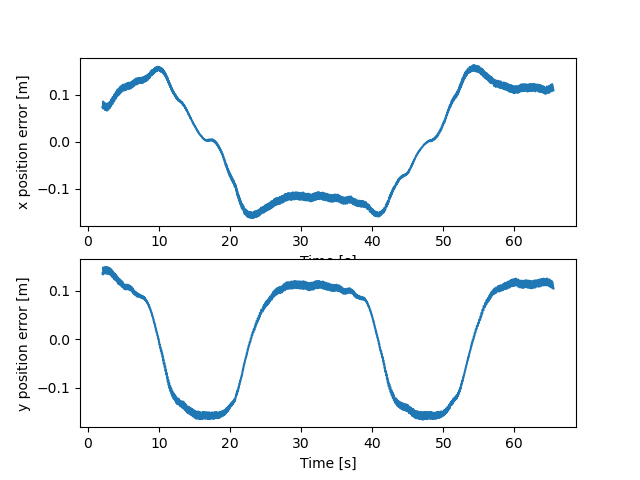
\includegraphics[scale=0.3]{img/dwa_screenshots/Position_Error.png}
\end{figure}

\end{columns}

\end{frame}

% * * * * * * * * * * * * * * * * * * * * * * * * * * * * * * * * * * * * * * *

\begin{frame}[allowframebreaks]
\frametitle{Comparison}

\vspace{-2em}

\begin{figure}[H]
    \centering
    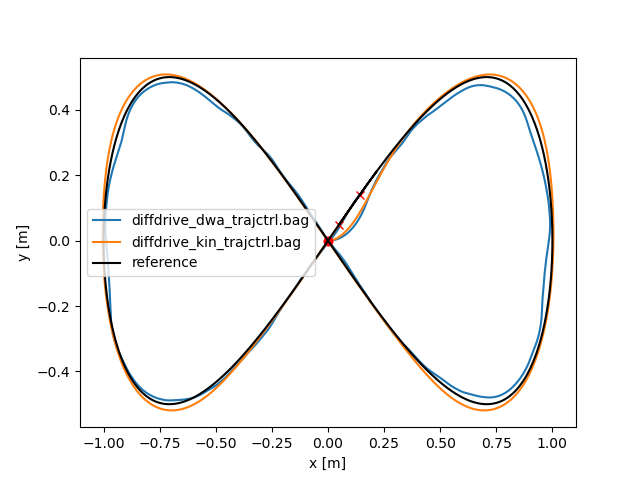
\includegraphics[scale=0.6]{img/comparison/Trajectory.png}
\end{figure}

\framebreak

\begin{columns}

\column{0.5\textwidth}

\vspace{-2em}

\begin{figure}[H]
    \centering
    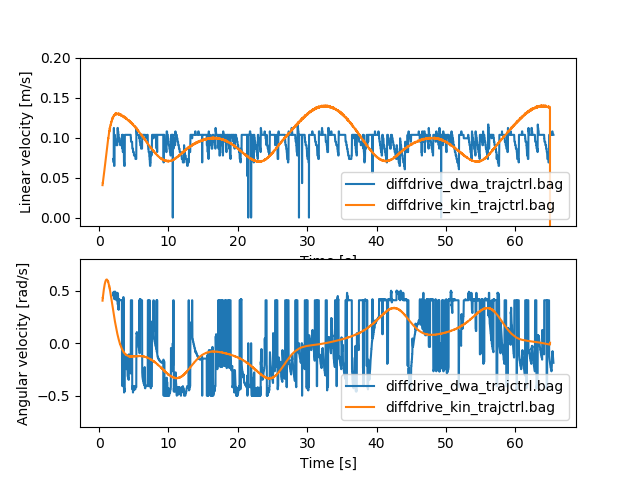
\includegraphics[scale=0.3]{img/comparison/Linear_and_Angular_Velocities.png}
\end{figure}

\vspace{-1em}

\begin{figure}[H]
    \centering
    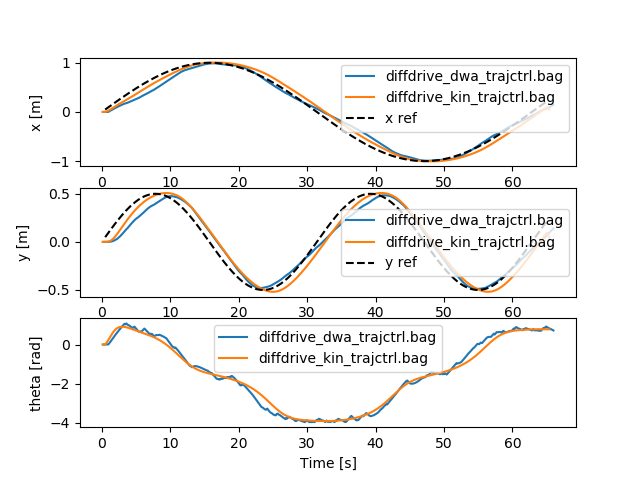
\includegraphics[scale=0.3]{img/comparison/Pose.png}
\end{figure}

\column{0.5\textwidth}

\vspace{-2em}

\begin{figure}[H]
    \centering
    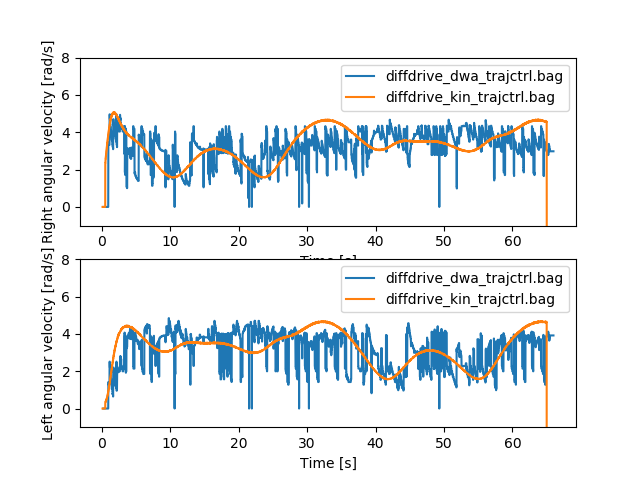
\includegraphics[scale=0.3]{img/comparison/Wheels_Velocities.png}
\end{figure}

\vspace{-1em}

\begin{figure}[H]
    \centering
    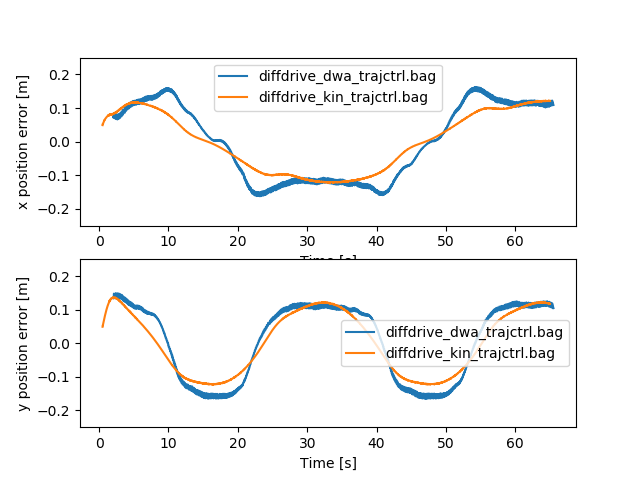
\includegraphics[scale=0.3]{img/comparison/Position_Error.png}
\end{figure}

\end{columns}

\end{frame}



%-----------------------------------------------------------------------------
%                                 FACED ISSUES
%-----------------------------------------------------------------------------

\section{Faced issues}

% * * * * * * * * * * * * * * * * * * * * * * * * * * * * * * * * * * * * * * *

\begin{frame}
\frametitle{Deprecated parameters}

There are some DWA parameters that are named differently between the ROS Wiki and
the library source code.

\vspace{1em}

\begin{figure}[H]
    \centering
    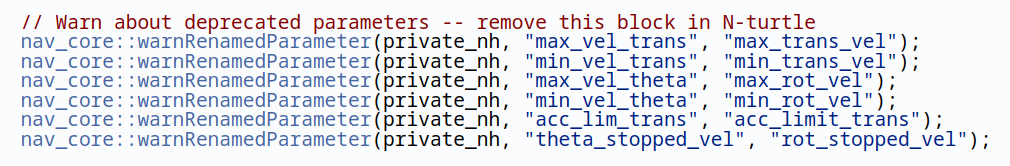
\includegraphics[scale=0.4]{img/other/deprecated_parameters_warning.png}
\end{figure}

\vspace{1em}

\begin{alertblock}{Unadvertised warning!}
Without using \texttt{nav\_core}, the warnings are not raised.
\end{alertblock}

\end{frame}

% * * * * * * * * * * * * * * * * * * * * * * * * * * * * * * * * * * * * * * *

\begin{frame}
\frametitle{DWA used standalone}

DWA expects information on certain topics (\texttt{/odom}, \texttt{/goal},
\texttt{/map}).
When used standalone, we must provide such information manually.

\vspace{2em}

Moreover, the few lines of code in the ROS Wiki explaining how to setup DWA
standalone are no longer working:

\begin{columns}

\column{0.4\textwidth}

\vspace{-1.5em}

\begin{figure}[H]
    \centering
    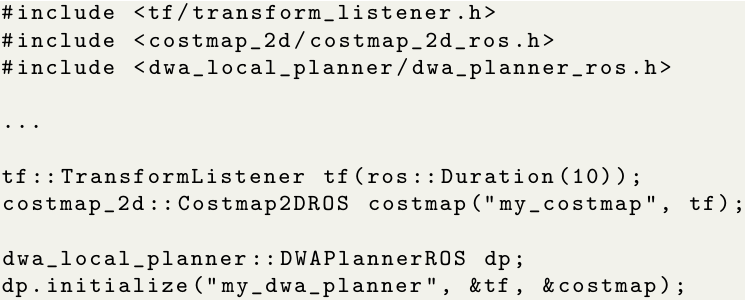
\includegraphics[scale=0.22]{img/other/old_dwa_snippet.png}
\end{figure}

\column{0.6\textwidth}

\begin{figure}[H]
    \centering
    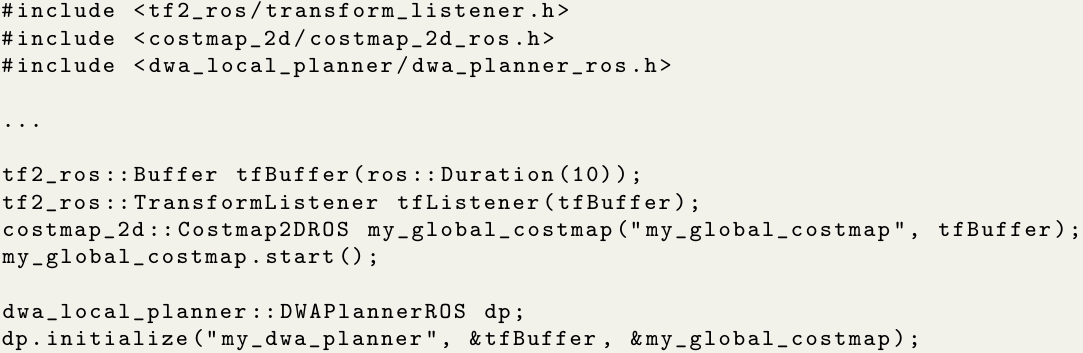
\includegraphics[scale=0.22]{img/other/new_dwa_snippet.png}
\end{figure}

\end{columns}

\end{frame}

% * * * * * * * * * * * * * * * * * * * * * * * * * * * * * * * * * * * * * * *

\begin{frame}
\frametitle{Multiple goals}

Generally, DWA takes only a single final goal and computes the full trajectory
on its own.

\vspace{2em}

In this project the trajectory is predefined and must be explicitly forced.
This is done by continuously changing the goal.

\vspace{2em}

We must find a suitable 'density' for the goals vector:
\begin{itemize}
  \item too many goals $\Rightarrow$ unsteady profile in the velocities
  \item too few goals $\Rightarrow$ large deviation from the reference trajectory
\end{itemize}

\end{frame}



%-----------------------------------------------------------------------------
%                                   CONCLUSION
%-----------------------------------------------------------------------------

\section{Conclusion}

% * * * * * * * * * * * * * * * * * * * * * * * * * * * * * * * * * * * * * * *

\begin{frame}
\frametitle{Conclusion}

Regarding the trajectory tracking aspect only, the two control methods behave
in a similar way even though the custom controller performs moderately better
than DWA.

\vspace{2em}

However, the most noticeable difference is in the smoothness of the plots of
linear and angular velocities: the custom controller produces velocities that
are much smoother and realistic than those produced by DWA.

\end{frame}



\end{document}

